\documentclass[12pt]{article}
\usepackage[pdfborder={0 0 0.5 [3 2]}, plainpages=false]{hyperref}%
\usepackage[left=1in,right=1in,top=1in,bottom=1in]{geometry}%
\usepackage[shortalphabetic]{amsrefs}%
\usepackage{amsmath}
\usepackage{enumerate}
% \usepackage{enumitem}
\usepackage{amssymb}                
\usepackage{amsmath}                
\usepackage{amsfonts}
\usepackage{amsthm}
\usepackage{bbm}
\usepackage[table,xcdraw]{xcolor}
\usepackage{tikz}
\usepackage{float}
\usepackage{booktabs}
\usepackage{svg}
\usepackage{mathtools}
\usepackage{cool}
\usepackage{url}
\usepackage{graphicx,epsfig}
\usepackage{makecell}
\usepackage{array}

\def\noi{\noindent}
\def\T{{\mathbb T}}
\def\R{{\mathbb R}}
\def\N{{\mathbb N}}
\def\C{{\mathbb C}}
\def\Z{{\mathbb Z}}
\def\P{{\mathbb P}}
\def\E{{\mathbb E}}
\def\Q{\mathbb{Q}}
\def\ind{{\mathbb I}}

\DeclareMathOperator{\spn}{span}
\DeclareMathOperator{\ran}{range}

\graphicspath{ {images/} }

\newtheorem{lemma}{Lemma}
\newtheorem{theorem}{Theorem}
\newtheorem{corollary}{Corollary}
\newtheorem{definition}{Definition}
\newtheorem{proposition}{Proposition}
\newtheorem{assumption}{Assumption}
\newtheorem{hypothesis}{Hypothesis}

\newtheorem{notation}{Notation}

\begin{document}

\section{Kink/antikinks in discrete Klein Gordon}

Reference is Kevrekidis and Weinstein (2000). Discrete Klein-Gordon equation
\[
\ddot{u_n} = d (\Delta_2 u)_n - f(u_n)
\]
where $\Delta_2$ is the discrete second difference operator. Versions we are interested in are discrete sine-Gordon, where $f(u) = \sin(u)$, and $\phi^4$ variant, where $f(u) = -2(u-u^3)$.

\subsection{Discrete sine-Gordon}
\[
\ddot{u_n} = d (\Delta_2 u)_n - \sin(u_n)
\]
Equilibrium solutions (standing waves) satisfy 
\[
d (\Delta_2 u)_n - \sin(u_n) = 0
\]
This has stable steady states $0, 2 \pi$ and unstable steady state $\pi$. Kinks are heteroclinic orbits connecting 0 to $2 \pi$, anti-kinks go the other way. Kinks known to exist (Kevrekidis and Weinstein, 2000), anti-kinks exist by symmetry. For an equilibrium solution $u_n$ (kink, etc.), eigenvalue problem is 
\[
d (\Delta_2 v)_n - \cos(u_n)v_n = \lambda^2 v_n
\]
Considered as an eigenvalue problem for $\lambda^2$, this is self-adjoint (symmetric, infinite dimensional matrix), so $\lambda^2$ is always real, which means that $\lambda$ must be either real or pure imaginary. 

Two distinctly kinks are possible, defined by what happens at AC limit.
\begin{itemize}
	\item intersite-centered: $(\dots, 0,0,0,2\pi,2\pi,2\pi,\dots)$
	\item onsite-centered: $(\dots, 0,0,0,\pi,2\pi,2\pi,\dots)$
\end{itemize}
Intersite-centered kink has a symmetric pair of imaginary eigenvalues which are well-separated from continuous spectrum (Goldstone mode) and two imaginary eigenvalues which abut the continuous spectrum (edge modes). Edge modes do not exist for all values of $d$. Goldstone mode eigenvalues approach 0 as $d \rightarrow \infty$, where they ``merge'' to form symmetry eigenvalue of continuum equation. Continuous spectrum is band on imaginary axis separated from origin.

\begin{figure}[H]
\begin{center}
\begin{tabular}{c}
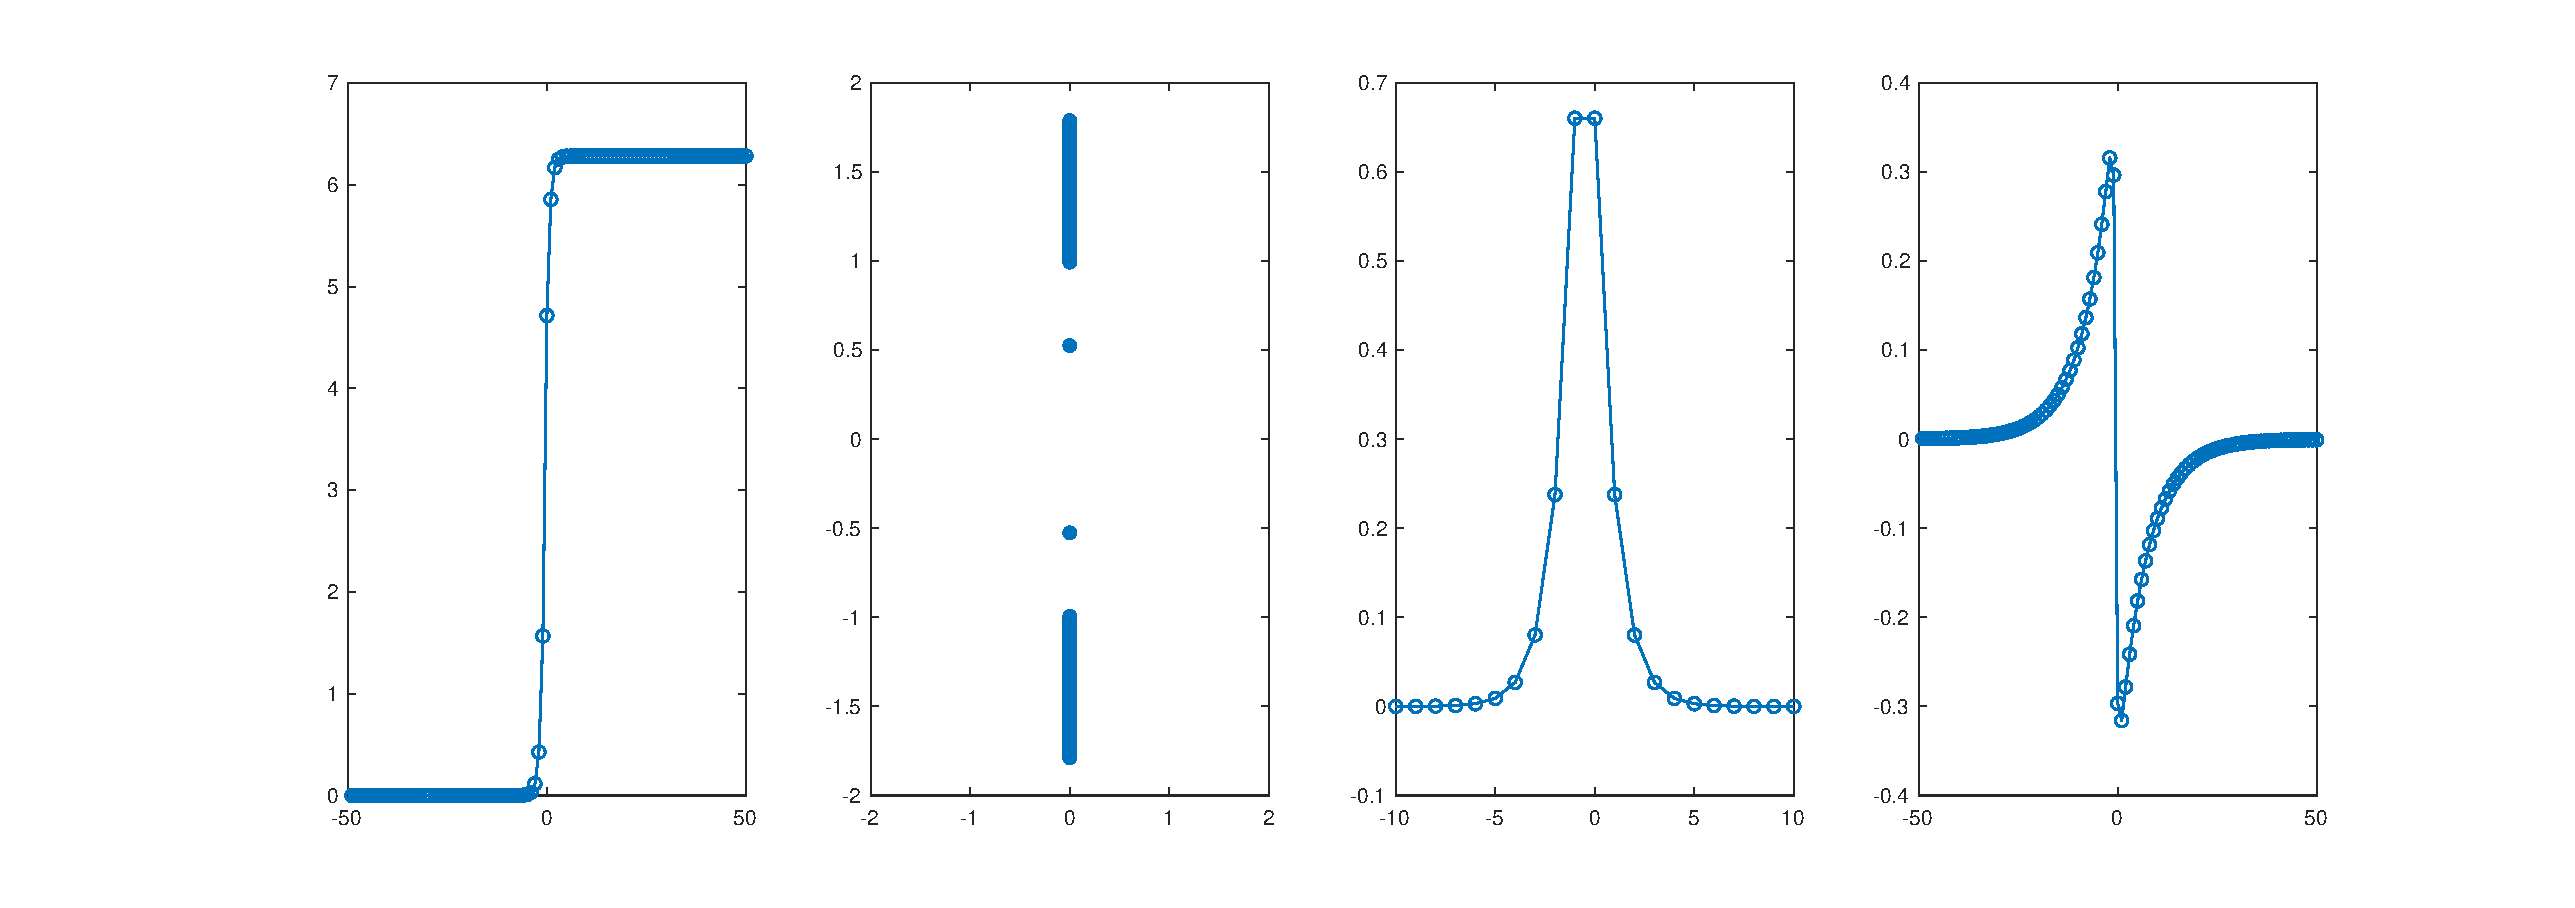
\includegraphics[height=4cm,width=15cm]{intersite.eps} \\
\end{tabular}
\end{center}
\caption{Intersite-centered kink. From left to right, plot of kink, spectrum, eigenfunction corresponding to Goldstone mode, and eigenfunction corresponding to edge mode. Goldstone mode eigenvalues $\lambda_g = \pm 0.5258i$. Edge mode eigenvalues $\lambda = 0.99438i$. Coupling constant $d = 0.55$. Generated from continuation from AC limit.}
\end{figure}

Onsite-centered incorporates the unsteady steady state in the middle of the kink. Onside-centered kink has a pair of real eigenvalues, so it is unstable. There does not appear to be an edge mode, at least not numerically. 
\begin{figure}[H]
\begin{center}
\begin{tabular}{c}
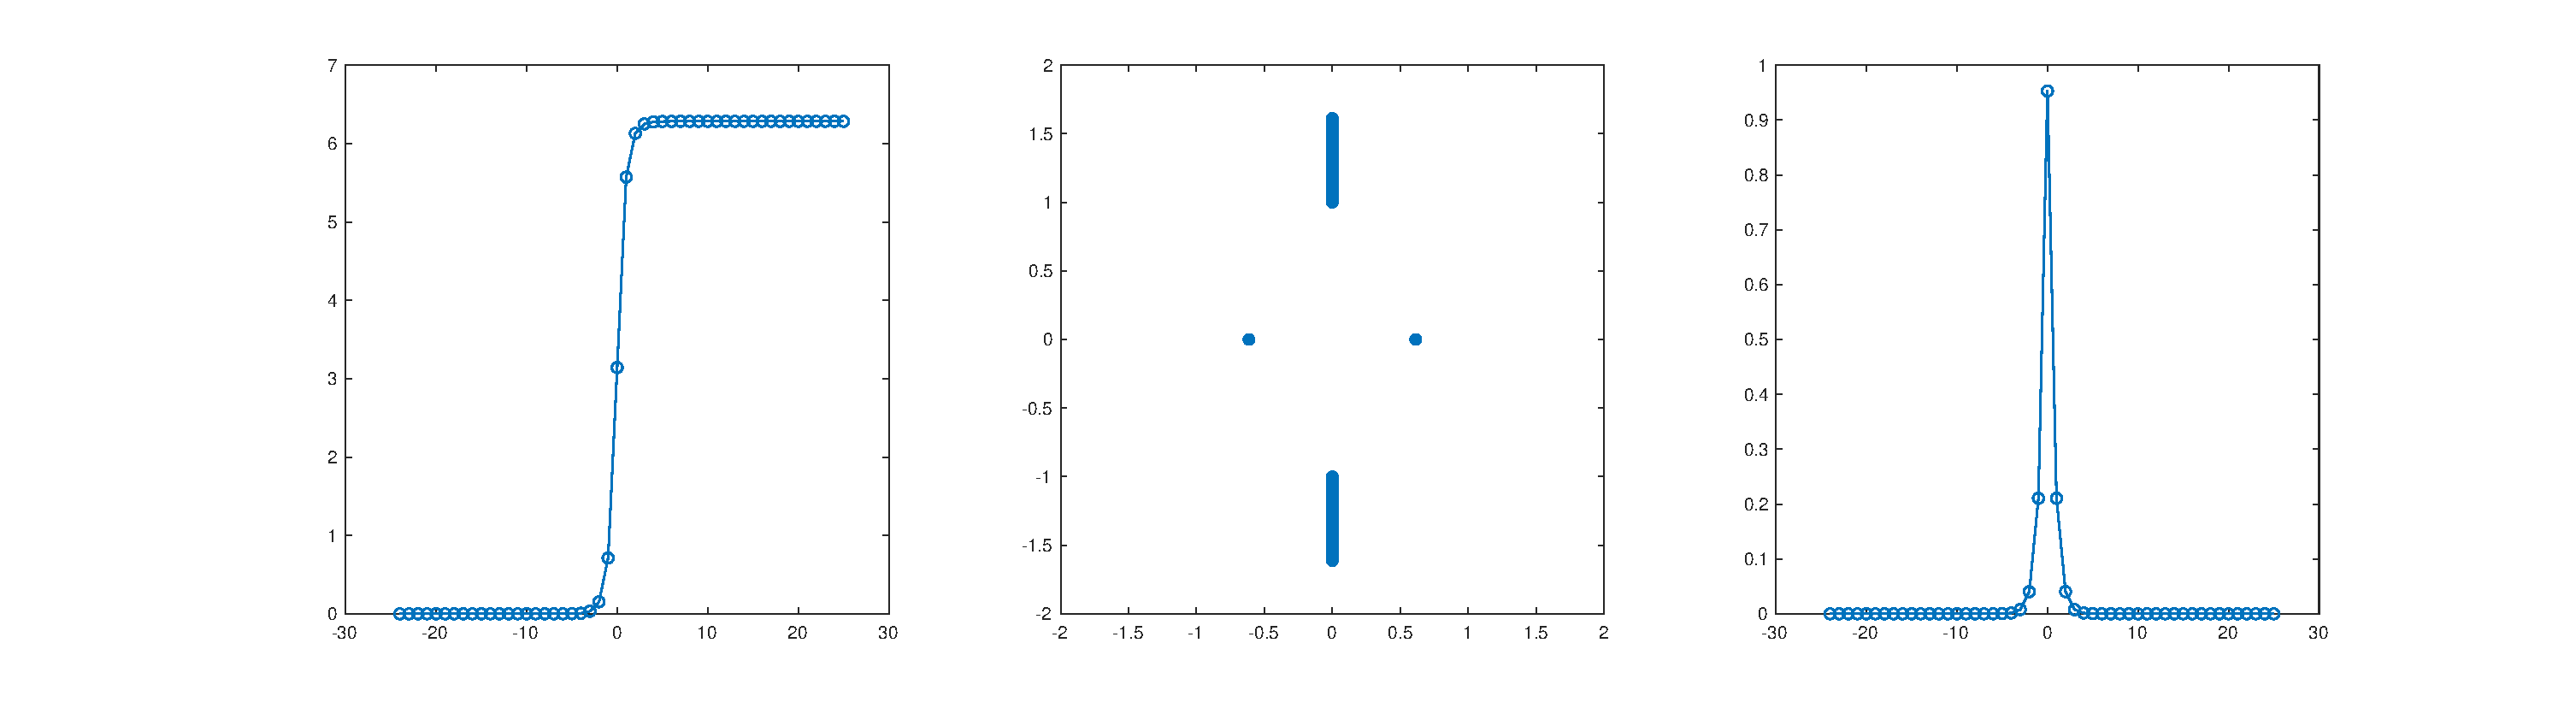
\includegraphics[height=4cm,width=15cm]{onsite.eps} \\
\end{tabular}
\end{center}
\caption{Onsite-centered kink. From left to right, plot of kink, spectrum, eigenfunction corresponding to real eigenvalue. Coupling constant $d = 0.40$. Generated from continuation from AC limit.}
\end{figure}

For kink-antikink interactions, we can splice together as many kinks and antikinks as we want. Numerically, we do this from parameter continuation from AC limit. We can do this for both intersite-centered and onsite-centered kinks (and can use a combination of both if we like), but here we only do intersite-centered ones (since the original kink is stable in that case). A single kink-antikink is like a double pulse, and each eigenvalue is doubled. We can keep playing this game. A kink-antikink-kink is like a triple pulse, and each eigenvalue is tripled, etc. The duplicated eigenvalues are ``exponentially close'' to those of the original kink.
\begin{figure}[H]
\begin{center}
\begin{tabular}{c}
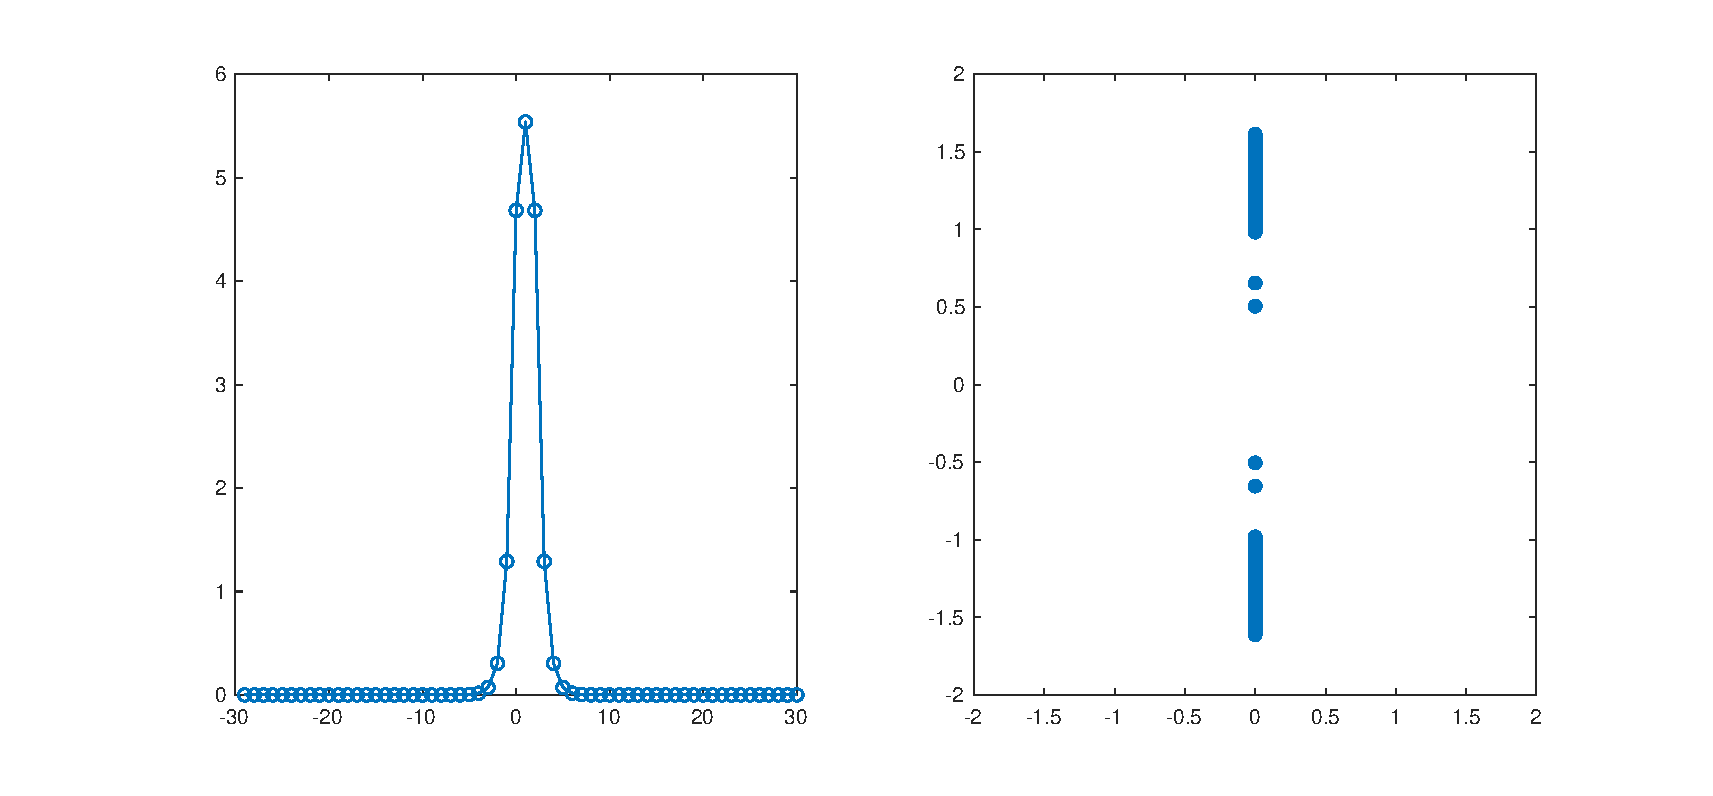
\includegraphics[height=4cm,width=10cm]{kinkantikink1.eps} \\
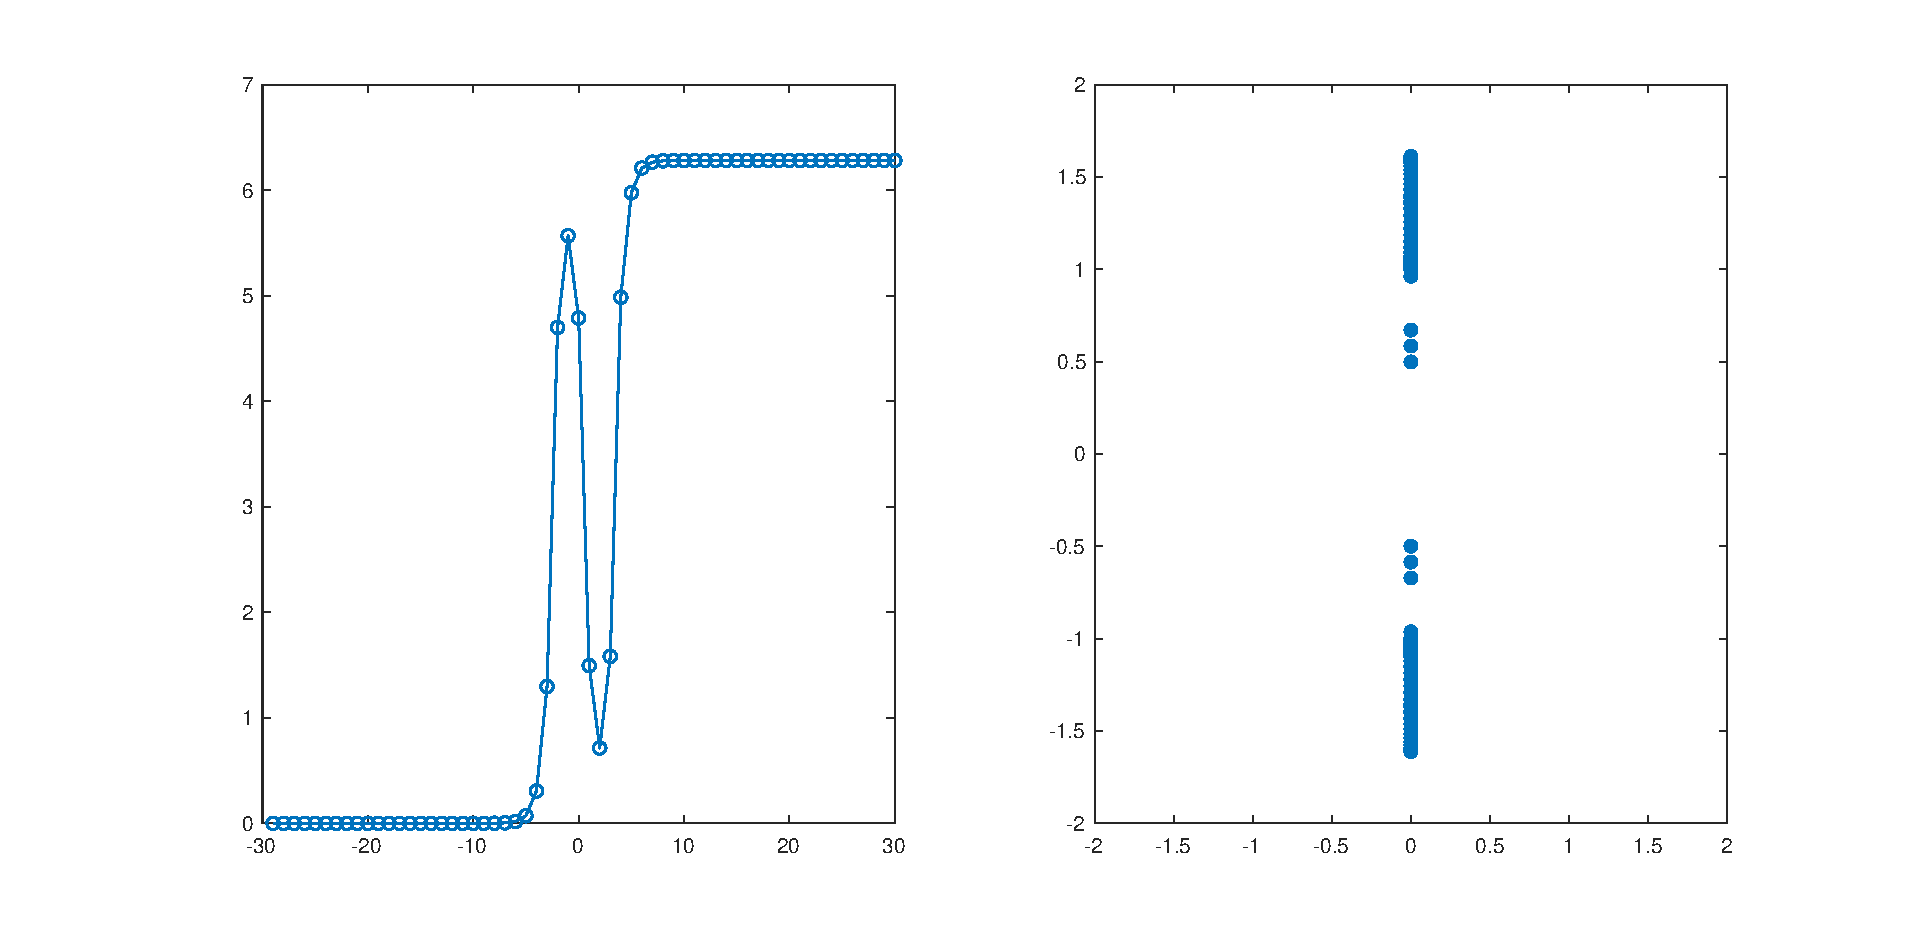
\includegraphics[height=4cm,width=10cm]{kinkantikinkkink1.eps} \\
\end{tabular}
\end{center}
\caption{Kink-antikink (top) and kink-antikink-kink (bottom) with onsite kinks with spectrum. Coupling constant $d = 0.4$. This shows doubling and tripling of the Goldstone mode. The edge mode also duplicates, but it is too close to the continuous spectrum to see in the plot.}
\end{figure}

To look at eigenfunctions of kink-antikink, we will make the kink and antikink ``well-separated''. We see that the dupicated eigenfunctions are approximately linear combinations (up-up and up-down) of the original kink eigenfunctions. This occurs for both the Goldstone mode and the edge mode. This suggests that we can construct both the kink-antikinks and these eigenfunctions with Lin's method.
\begin{figure}[H]
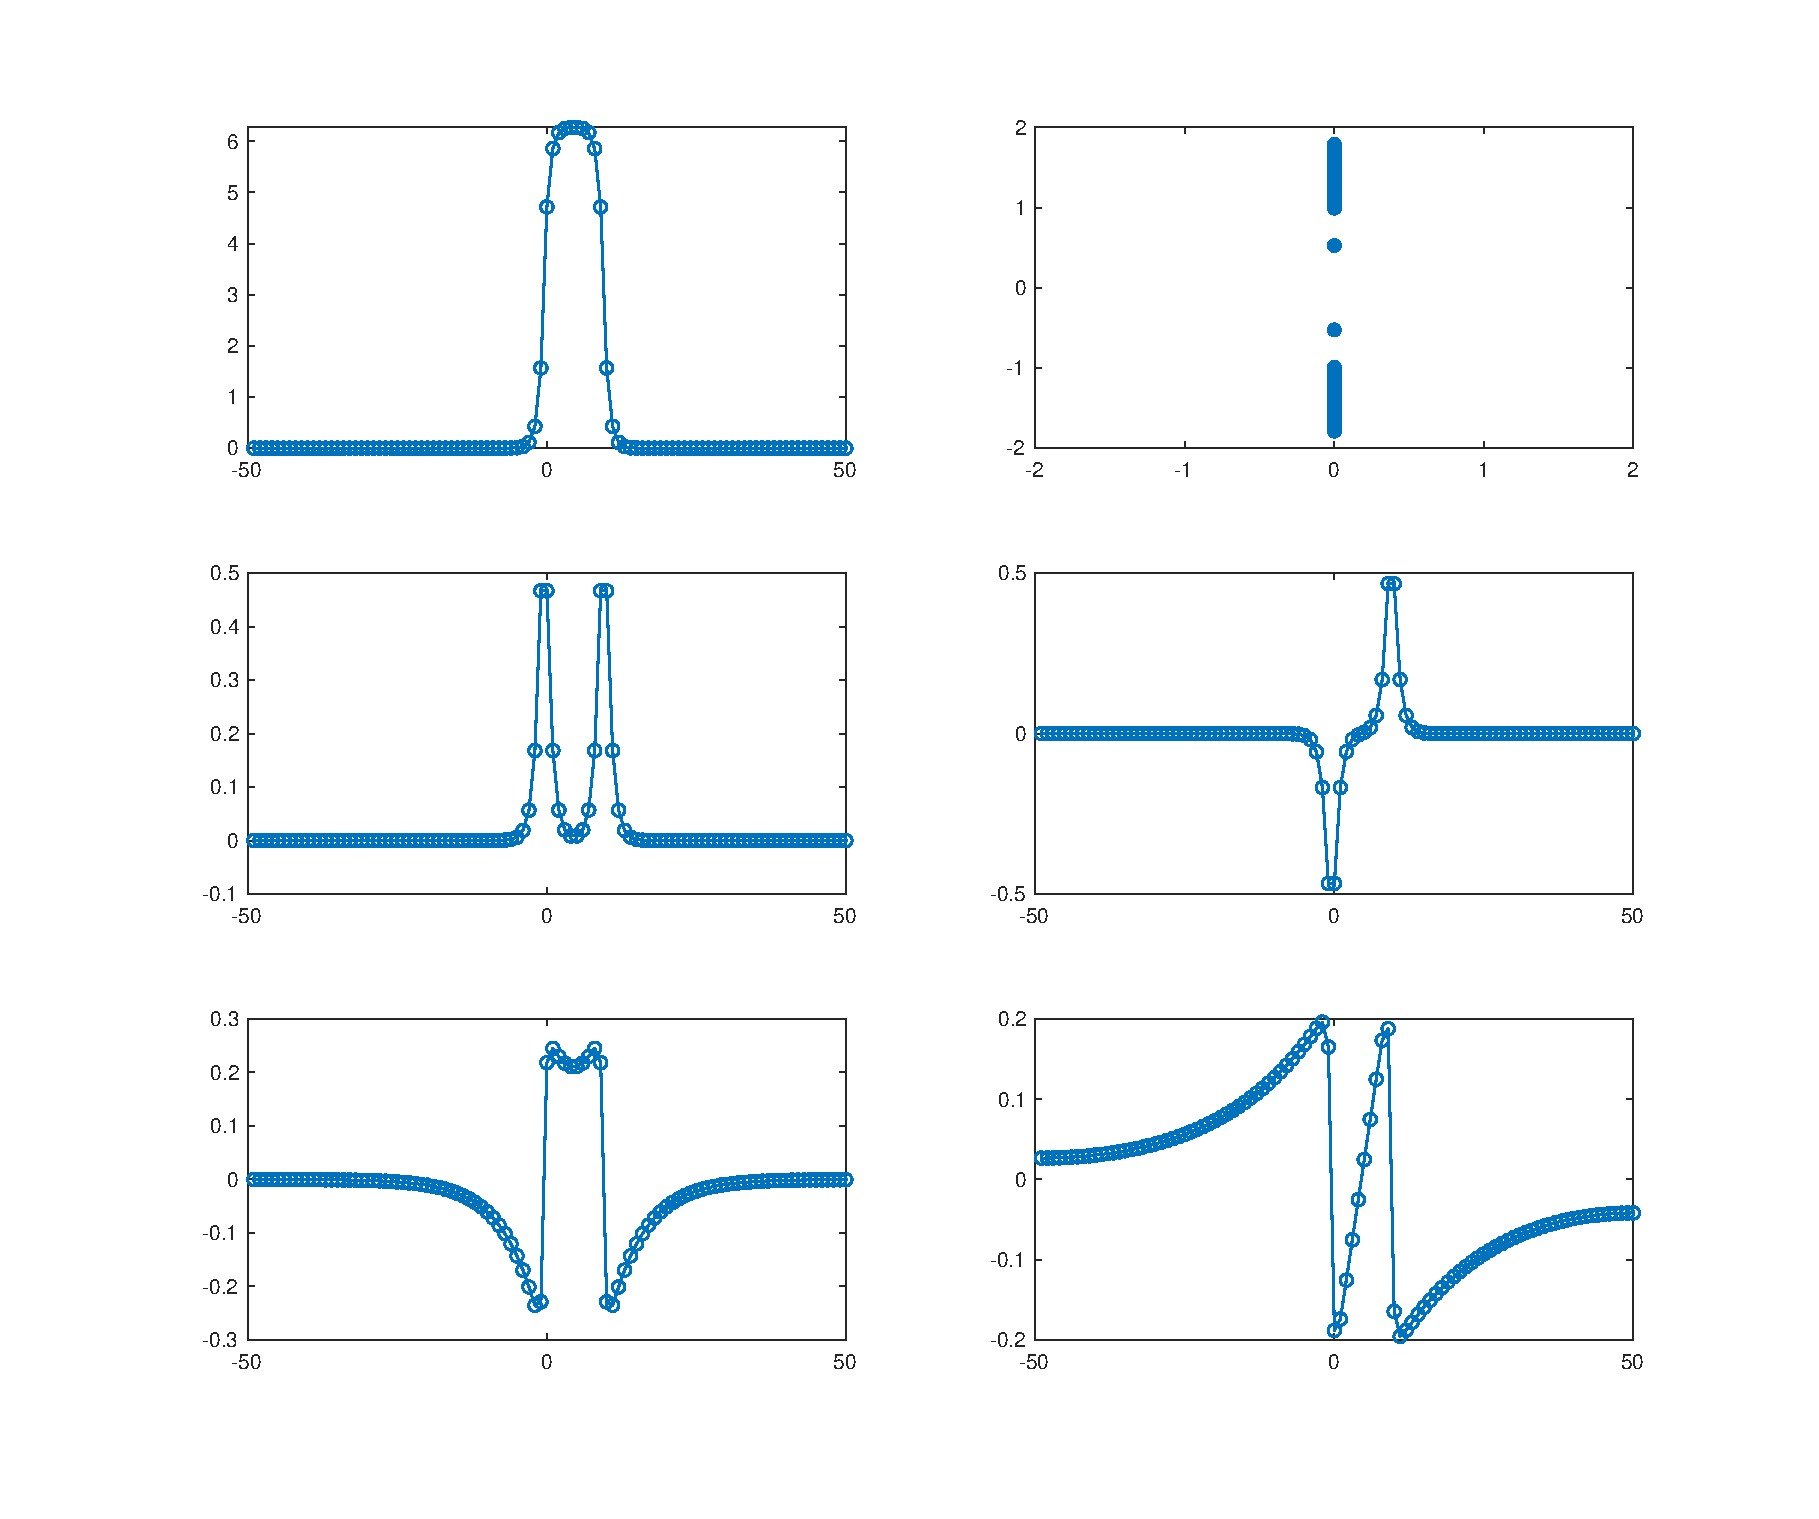
\includegraphics[width=17cm]{kinkantikink2.eps} \\
\caption{Kink-antikink and spectrum. Eigenfunctions for doubled Goldstone mode (middle). Eigenfunctions for doubled edge mode (bottom). Coupling constant $d = 0.55$.}
\end{figure}

\subsection{Discrete $\phi^4$}

Exactly the same thing happens, except the initial kink can also have another imaginary eigenmode (shape mode), which also duplicates.


\end{document}